%%%%%%%%%%%%%%%%%%%%%%%%%%%%%%%%%%%%%%%%%%%%%%%%%%%%%%%%%% 
\chapter{実行実験}\label{chap:experiment}
%%%%%%%%%%%%%%%%%%%%%%%%%%%%%%%%%%%%%%%%%%%%%%%%%%%%%%%%%% 

本章では,前章で提案した3つの符号化
\textsf{undirected},\textsf{directed},\textsf{acyclicity}
の性能を評価するために実行実験を行った.
%
実験に使用したベンチマーク問題集(計494問)は,以下の通りである.
\begin{itemize}
\item \textsf{color04} (計127問)\\
  グラフ彩色問題の国際競技会
  COLOR02/03/04~\footnote{\url{https://mat.tepper.cmu.edu/COLOR02/}}
  で使用された問題インスタンス.
\item \textsf{complete} (計15問)\\
  SATソルバーを用いた既存研究~\cite{soh14:jelia2014}で提供された
  完全グラフのインスタンス~\footnote{\url{https://tsoh.org/scarab/jelia2014/}}.
\item \textsf{knight} (計11問)\\
  $N\times N$の騎士巡回問題(Knight's Tour)のインスタンス.\\
  $N=8,12,20,30,40,50,60,70,80,90,100$の11通り.
\item \textsf{tsplib} (9問)\\
  巡回セールスマン問題のポータルサイトTSPLIBに公開されている
  インスタンス\footnote{\url{http://comopt.ifi.uni-heidelberg.de/software/TSPLIB95/hcp/}}.
\item \textsf{grid} (12問)\\
  $N$次の正方グリッドグラフのインスタンス($6\leq N\leq 17$).
\item \textsf{random} (320問)\\
  SATソルバーを用いた既存研究~\cite{soh14:jelia2014}で提供された
  ランダムグラフのインスタンス~\footnote{\url{https://tsoh.org/scarab/jelia2014/}}.
\end{itemize}

使用した ASP システムは{\clingo}のバージョン5.4.0である.
オプションには,\textit{trendy}と\textit{crafty}を使用した.
一問あたりの時間制限は30分とした.
実験環境は,Mac mini Intel Corei7 3.2GHz 64GBメモリである.

%%%%%%%%%%%%%%%%%%%%%%%%%%%%%%%%%%%%%%%%%%%%%%%%%%%%%%%%%%
\section{ハミルトン閉路問題の実験結果}
%%%%%%%%%%%%%%%%%%%%%%%%%%%%%%%%%%%%%%%%%%%%%%%%%%%%%%%%%%

%%%%%%%%%%%%%%%%%%%%%%%%%%%%%%%%%%%%%%%%%%%%%%%
\begin{table}[t]\scriptsize
  \centering
  %\tabcolsep = 0.8mm
  \renewcommand{\arraystretch}{1.2}
  \begin{tabular}{lr|rrr}
    問題サイズ & 問題数 & \textsf{undirected} & \textsf{directed} & \textsf{acyclicity}\\
   \hline
    $\:\:\:\:\:\,\, 0 \leq |V| < 1000$     & 171   & 156   & \alert{171}   & 156  \\ %
    $1000 \leq |V| < 2000$  & 165   & 120   & \alert{159}   & 121  \\
    $2000 \leq |V| < 3000$  & 177   & 125   & \alert{163}   & 80   \\
    $3000 \leq |V| < 4000$  & 185   & 104   & \alert{147}   & 48   \\
    $4000 \leq |V| < 5000$  & 128   & 92    & \alert{106}   & 30   \\
    $5000 \leq |V| < 6000$  & 80    & 63    & \alert{70}    & 21   \\
    $6000 \leq |V| < 7000$  & 55    & 39    & \alert{41}    & 20   \\
    $7000 \leq |V| < 8000$  & 28    & 12    & \alert{15}    & 4    \\
    $8000 \leq |V| < 9000$  & 10    & 2     & \alert{5}     & 1    \\
    $9000 \leq |V| < 10000$  & 2     & \alert{2}     & \alert{2}     & 1    \\
   \hline
    合計 & 1001 & 715   & \alert{879}   & 482  
  \end{tabular}
  \vskip .5em
%  \caption{ハミルトン閉路問題: 解けた問題数}
  \label{sat_table}
\end{table}
%label{sat_table}
%%%%%%%%%%%%%%%%%%%%%%%%%%%%%%%%%%%%%%%%%%%%%%%

%%%%%%%%%%%%%%%%%%%%%%%%%%%%%%%%%%%%%%%%%%%%%%%
\begin{figure}[tb]
\begin{center}
  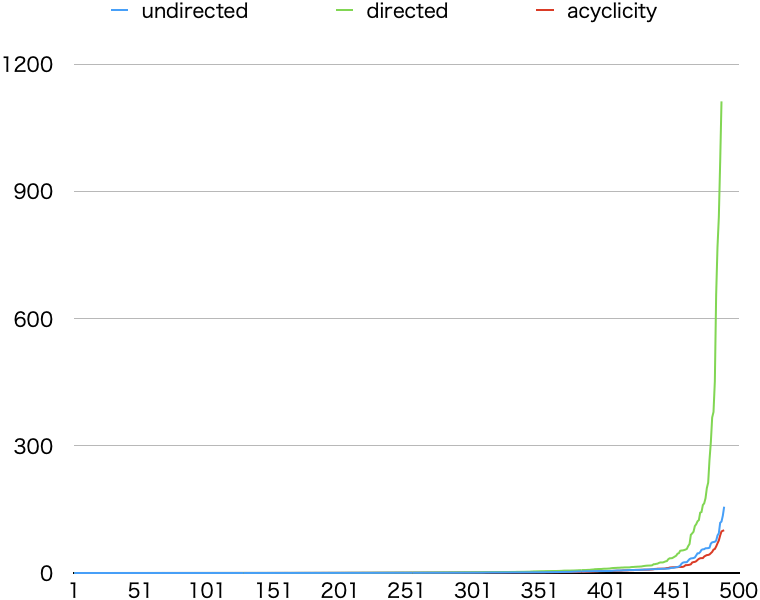
\includegraphics[width=0.6\linewidth]{fig/cactus.png}
\caption{ハミルトン閉路問題: カクタスプロット (\textsf{SAT+UNSAT})}
\label{cactus}
\end{center}
\end{figure}
%%%%%%%%%%%%%%%%%%%%%%%%%%%%%%%%%%%%%%%%%%%%%%%

%%%%%%%%%%%%%%%%%%%%%%%%%%%%%%%%%%%%%%%%%%%%%%%
\begin{figure}[tb]
\begin{center}
  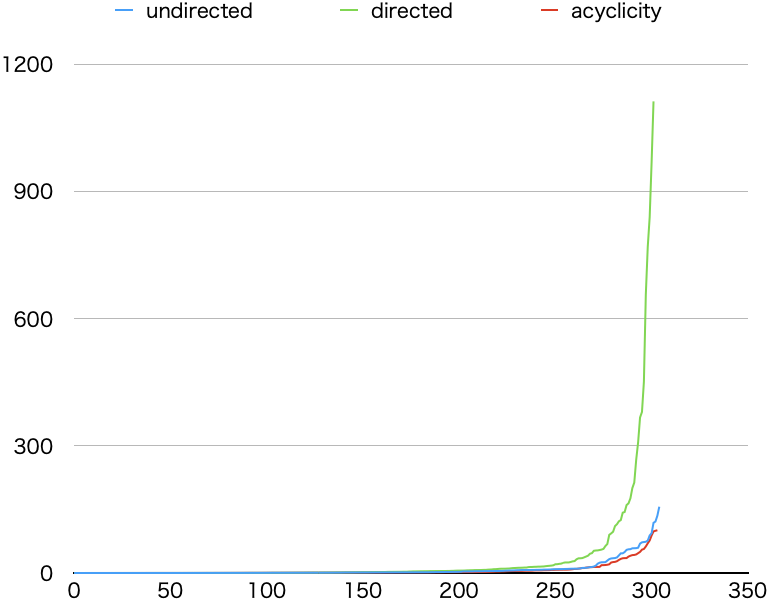
\includegraphics[width=0.6\linewidth]{fig/cactussat.png}
\caption{ハミルトン閉路問題: カクタスプロット (\textsf{SAT})}
\label{cactussat}
\end{center}
\end{figure}
%%%%%%%%%%%%%%%%%%%%%%%%%%%%%%%%%%%%%%%%%%%%%%%

%%%%%%%%%%%%%%%%%%%%%%%%%%%%%%%%%%%%%%%%%%%%%%%
\begin{figure}[tb]
\begin{center}
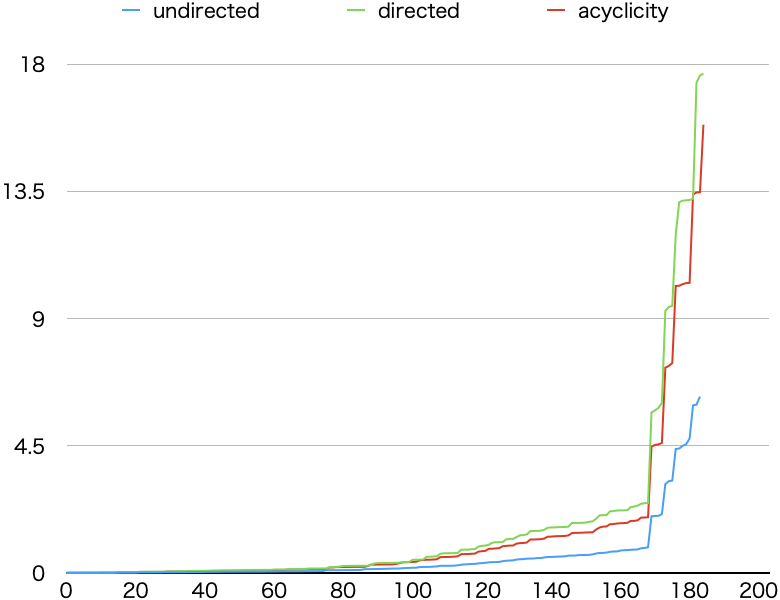
\includegraphics[width=0.6\linewidth]{fig/cactusunsat.png}
\caption{ハミルトン閉路問題: カクタスプロット (\textsf{UNSAT})}
\label{cactusunsat}
\end{center}
\end{figure}
%%%%%%%%%%%%%%%%%%%%%%%%%%%%%%%%%%%%%%%%%%%%%%%

%--
表~\ref{sat_table}に,各符号化で解けた問題数を示す.
ベンチマーク問題の種類ごとに,
\textsf{SAT},
\textsf{UNSAT},
\textsf{SAT+UNSAT},...


\textsf{SAT+UNSAT}の問題数については,xxxxx だった.

\textsf{SAT}の問題数については,xxxxx だった.

\textsf{UNSAT}の問題数については,xxxxx だった.


%--
図~\ref{cactus}に,\textsf{SAT+UNSAT}のカクタスプロットを示す.
縦軸は問題を解くのに要した CPU 時間,横軸は解けた問題数を表す.
グラフが右によるほど多くの問題を解けたことを示し,
下によるほどより速く解けたことを示す.
図~\ref{cactus}より,\textsf{acyclicity}符号化は,解けた問題数が同じ
\textsf{undirected}符号化と比較して,より高速に問題を説いていることが
確認できた.

次に,図~\ref{cactussat}と図~\ref{cactusunsat}に,
\textsf{SAT}と\textsf{UNSAT}のカクタスプロットを示す.
図~\ref{cactussat}より,\textsf{SAT}のみの場合は,
\textsf{SAT+UNSAT}と比べて,符号化の優劣に差は見られなかった.
一方で,
図~\ref{cactusunsat}から,xxxxxxxx,yyyy


%--
% \item 結果に差が生じた2問について,color04の問題は解がSATであったが,
%   gridの問題の解はUNSATであった.
%\item color04にて,\textsf{undirected}に解けて\textsf{acyclicity}に解けなかった問題では,変数の個数や一貫性制約の数において,その結果に反して\textsf{acyclicity}が少ない値を示したに.
%\item しかし,{\clingo}が解く過程で\textsf{acyclicity}では,制限時間内のみで,\textsf{undirected}の約40倍もの選択が行われ,発生したコンフリクト数は約60倍であった.
%\item 一方で,gridにて\textsf{acyclicity}に解けて\textsf{undirected}に解けなかった問題では,一貫性制約の数に大きな差はなかったが,変数の数において後者は前者の2倍であった.
%\item さらに,{\clingo}が解く過程で発生した選択数は後者は前者の90倍以上であった.


%%%%%%%%%%%%%%%%%%%%%%%%%%%%%%%%%%%%%%%%%%%%%%%%%%%%%%%%%%
\section{最短ハミルトン閉路問題}
%%%%%%%%%%%%%%%%%%%%%%%%%%%%%%%%%%%%%%%%%%%%%%%%%%%%%%%%%%

%%%%%%%%%%%%%%%%%%%%%%%%%%%%%%%%%%%%%%%%%%%%%%%
\begin{table}[htbp]
  \caption{実験結果2-1:trendy}
  \label{min_table_tr}
  \centering
  \begin{tabular}{|l|rrr|}
    \hline
    Instance&undirected&directed&acyclicity \\
    \hline
    grid5&50,656*&50,656*&50,656* \\
    grid6&68,656*&68,656*&68,656* \\
    grid7&91,822*&91,822*&91,822* \\
grid8&113,250&\textcolor{red}{112,916}&113,277 \\
grid9&\textcolor{red}{142,502}&143,326&143,660 \\
grid10rc&\textcolor{red}{172,703}&174,866&175,999 \\
grid11&\textcolor{red}{200,399}&204,456&200,638 \\
grid12&\textcolor{red}{231,278}&239,275&232,012 \\
grid13&\textcolor{red}{276,692}&276,926&276,899 \\
grid14&317,617&\textcolor{red}{317,144}&317,676 \\
grid15&\textcolor{red}{375,906}&376,809&376,210 \\
grid16&421,249&\textcolor{red}{419,737}&423,753 \\
US48&11,698*&11,698*&11,698* \\
    \hline
  \end{tabular}
\end{table}
%\label{min_table_tr}
%%%%%%%%%%%%%%%%%%%%%%%%%%%%%%%%%%%%%%%%%%%%%%%

この節では,提案した3つのASP符号化
\textsf{undirected},\textsf{directed},\textsf{acyclicity}の
最短ハミルトン閉路問題に対しての性能を比較評価する.

\begin{itemize}
\item ベンチマーク問題としては,12個の正方グリッドグラフと図~\ref{fig:USmap}の米国本土48州の隣接グラフを用いた.
\item 12個の正方グリッドグラフは,前節で用いたgridと同じものである.
\item グリッドグラフの各辺のコストは1000〜2000の範囲の一様ランダム整数値である.
\end{itemize}

解くのに使用したASPシステムは{\clingo}のver5.4.0であり,
オプションは\textit{trendy},一問あたりの時間制限を3時間とした.
実験環境は,Mac mini Intel Corei7 3.2GHz 64GBメモリである.

実験結果を表~\ref{min_table_tr}にまとめた.

\begin{itemize}
\item 表~\ref{min_table_tr}は,制限時間内に求められたハミルトン閉路の最短距離をまとめたものである.
\item 赤文字が,3符号化を比較した際の最良値であり,*マークがその問題の最短距離が求められたことを表している.
\item したがって,grid5〜7とUS48では全ての符号化にて最短距離が時間内に求められた.
\item 表~\ref{min_table_tr}より,赤文字がもっとも多かった\textsf{undirected}が優秀な性能を示した.
\end{itemize}

%%%%%%%%%%%%%%%%%%%%%%%%%%%%%%%%%%%%%%%%%%%%%%%%%%%%%%%%%%
\section{コスト制約付きハミルトン路問題}
%%%%%%%%%%%%%%%%%%%%%%%%%%%%%%%%%%%%%%%%%%%%%%%%%%%%%%%%%%

%%%%%%%%%%%%%%%%%%%%%%%%%%%%%%%%%%%%%%%%%%%%%%%
\begin{table*}[tb]\footnotesize
  \tabcolsep = 2mm
  %\renewcommand{\arraystretch}{1.0}
  \vskip .5em
  \centering
  \begin{tabular}{lr|rrr}
    \hline
    閾値(倍率)    &	解の総数 & \textsf{undirected} & \textsf{directed} & \textsf{acyclicity} \\
    \hline
    11698(1.00)   &	1      &\textbf{2.979} & 7.531 & 4.586	\\
    11814(1.01)   &	8      &5.587  & 15.322	& \textbf{5.250}	\\
    11931(1.02)   &	28     &\textbf{3.243}& 18.600	& 3.578	\\
    12282(1.05)   &	388    &10.003&19.818	& \textbf{6.296}	\\
    12867(1.10)   &	16,180  &16.548& 28.555	& \textbf{9.764}\\
    14037(1.20)   &	939,209 &48.262       &40.717	& \textbf{26.837}\\
    15207(1.30)   &	4,525,541&88.172      &55.276	& \textbf{42.037}\\
    16377(1.40)   &	6,702,964&99.154       &47.647	& \textbf{40.640}	\\
    17547(1.50)   &	6,876,526&95.390       &45.265	& \textbf{38.411}	\\
    18716(1.60)   &	6,876,928&98.937       &49.138	& \textbf{40.748}	\\
    \hline
    平均CPU時間 &   & 46.8275 & 32.7869  & \textbf{21.8147}\\\hline
%    Best    &   & 2 & 0 & \textbf{8} \\ \hline
  \end{tabular}
  \vskip .5em
  \caption{コスト制約付きハミルトン路問題: 解の全列挙に要した CPU 時間}
  \label{cost_table}
\end{table*}
%\label{cost_table}
%%%%%%%%%%%%%%%%%%%%%%%%%%%%%%%%%%%%%%%%%%%%%%%

この節では,提案した3つのASP符号化
\textsf{undirected},\textsf{directed},\textsf{acyclicity}の
コスト制約付きハミルトン閉路問題に対しての性能を比較評価する.

\begin{itemize}
\item ベンチマーク問題として図~\ref{fig:USmap}の米国本土48州の隣接グラフを用いた.
\item 閾値は表\ref{cost_table}にあるように11698〜18716までの10の値を与えた.
\item 始点はWA,終点はMEとした.
\end{itemize}

解くのに使用したASPシステムは{\clingo}のver5.4.0であり,
オプションは\textit{crafty},一問あたりの時間制限を3時間とした.
実験環境は,Mac mini Intel Corei7 3.2GHz 64GBメモリである.

実験結果として,表~\ref{cost_table}に問題ごとにかかったCPU時間と解の個数をまとめた.

\begin{itemize}
\item 表~\ref{cost_table}では,各閾値におけるコスト制約を満たした
  ハミルトン路の数がModelsの列に記されており,
  その右に各符号化が解くのにかかったCPU時間が記されている.
\item 赤文字が3符号化の中での最短時間を表しており,タイムアウトは発生しなかった.
\item 10の閾値の内の7つにて\textsf{acyclicity}が最短時間で解いている.
\item 各閾値でかかったCPU時間の平均でも,\textsf{acyclicity}が最小である.
\item \textsf{acyclicity}がもっとも優秀であった.
\end{itemize}
%%%%%%%%%%%%%%%%%%%%%%%%%%%%%%%%%%%%%%%%%%%%%%%%%%%%%%%%%%

%%% Local Variables:
%%% mode: latex
%%% TeX-master: "paper"
%%% End:
